\chapter{Finding Ambiguity from Disagreement}
\label{chap:frames}
\addcontentsline{lof}{chapter}{\textsc{Chap.~\ref{chap:frames}: Finding Ambiguity from Disagreement}}
\addcontentsline{lot}{chapter}{\textsc{Chap.~\ref{chap:frames}: Finding Ambiguity from Disagreement}}


%\begin{chapquote}{Douglas Adams, \textsc{The Hitchhiker's Guide to the Galaxy}}
%We demand rigidly defined areas of doubt and uncertainty!
%\end{chapquote}

% \begin{chapquote}{Friedrich Nietzsche, \textsc{Notebooks (Summer 1886 – Fall 1887)}}
% Against that positivism which stops before phenomena saying ``there are only facts,'' I should say: no, it is precisely facts that do not exist, only interpretations.
% \end{chapquote}

\begin{chapquote}{Bertrand Russell, \textsc{The Philosophy of Logical Atomism}}
Everything is vague to a degree you do not realize until you have tried to make it precise, and everything precise is so remote from everything that we normally think, that you cannot for a moment suppose that is what we really mean when we say what we think.
\end{chapquote}


In this chapter, we investigate how inter-annotator disagreement can be used as an indicator for language ambiguity, using the task of FrameNet frame disambiguation as a use case. FrameNet is a computational linguistics resource composed of semantic frames, high-level concepts that represent the meanings of words. In this chapter, we present an approach to gather frame disambiguation annotations in sentences using a crowdsourcing approach with multiple workers per sentence to capture inter-annotator \emph{disagreement}. We perform an experiment over a set of 433 sentences annotated with frames from the FrameNet corpus, and show that the aggregated crowd annotations achieve an F1 score greater than 0.67 as compared to expert linguists. . This methodology was then scaled up to collect a frame disambiguation resource over 5,000 sentence-word pairs from Wikipedia -- the largest corpus of this type outside of FrameNet.

A qualitative examination of the disagreement in our data revealed cases where the crowd annotation was correct even though the expert is in disagreement, arguing for the need to have multiple annotators per sentence. Most importantly, we examine cases in which crowd workers could not agree, and demonstrate that these cases exhibit ambiguity, either in the sentence, frame, or the task itself, and argue that collapsing such cases to a single, discrete truth value (i.e. correct or incorrect) is inappropriate, creating arbitrary targets for machine learning.

This chapter is based on the following publications:
\begin{itemize}
    \item \textit{Capturing Ambiguity in Crowdsourcing Frame Disambiguation}, in the AAAI Conference on Human Computation and Crowdsourcing, co-authored by Lora Aroyo and Chris Welty~\cite{DBLP:conf/hcomp/DumitracheAW18};
    
    \item \textit{A Crowdsourced Frame Disambiguation Corpus with Ambiguity}, in submission, co-authored by Lora Aroyo and Chris Welty.
\end{itemize}


\section{Introduction}

% \textbf{RQ4:} \textit{Is inter-annotator disagreement an accurate indicator for ambiguity in natural language?}

We have shown that preserving inter-annotator disagreement can result in ground truth data of a high quality (Chapters~\ref{chap:med-rel-ex} \&~\ref{chap:maj-vote}), that can be used to improve the performance of natural language processing systems (Chapter~\ref{chap:od-rel-ex}). Based on these results, it appears that inter-annotator disagreement is a useful property to have in ground truth data. We argue that is because \textit{disagreement is often times indicative of ambiguity that is inherent to natural language} (\textbf{RQ4}). In this chapter, we explore how disagreement can be used as an indicator for language ambiguity, using the task of FrameNet frame disambiguation as a use case.

FrameNet is a computational linguistics resource based on the frame semantics theory~\cite{baker1998berkeley}. A semantic \textit{frame} is an abstract representation of a word sense, describing a type of entity, relation, or event, and identifies the associated \emph{roles} implied by the frame. The FrameNet resource offers a collection of semantic frames, together with a corpus of documents annotated with these frames. In the corpus, individual words are mapped to the single frame that represents the meaning of that word in the sentence.  

Since many words have multiple possible meanings, the task of obtaining these annotations is called \emph{frame disambiguation}, similarly to word-sense disambiguation.  It is a complex task that typically is performed by linguistic experts, subjected to strict annotation guidelines and quality control~\cite{baker2012framenet}. As such, this task typically does not scale sufficiently in order to meet the annotation requirements of modern machine learning methods. Moreover, the annotation is typically performed by only one expert, which makes it impossible to capture any diversity of perspectives.  

There have been a number of attempts at using crowdsourcing for frame disambiguation in sentences, such as those by \citet{Hong:2011:GCR:2018966.2018970} and \citet{chang2015scaling}, offering a creative way to deal with the complexity of the annotation task. This chapter addresses the considerable problem of \emph{ambiguity}  in frame annotation, which we show to be a prominent feature in frame semantics.  We adapt the CrowdTruth framework, which encourages using multiple crowd annotators to perform the same work, and processes the disagreement between them to signal low quality workers, sentences, and frames.

This chapter presents the following contributions:

\begin{enumerate}

\item \emph{metrics for frame and sentence quality}: a qualitative evaluation showing that inter-annotator disagreement is an indicator of ambiguity in both frames and sentences (Section~\ref{sec:frame-metrics});

\item \emph{crowd vs. expert evaluation}: the crowd achieves comparative quality with trained FrameNet experts (F1 $>0.67$), and we provide examples of typical cases where the crowd annotation is correct despite the expert disagreement (Section~\ref{sec:frame-crowd-exp});

\item \emph{ambiguity-aware annotation methodology}: we demonstrate that the cases in which the crowd workers could not agree exhibit ambiguity, either in the sentence, frame, or the task itself; we argue that collapsing such cases to a single, discrete truth value (i.e. correct or incorrect) is inappropriate, creating arbitrary targets for machine learning (Section~\ref{sec:frame-ambig});

\item \emph{evaluation of several frame disambiguation models}: using evaluation metrics that leverage the multiple possible frames per sentence and their confidence scores, we show that even a model that always predicts the top crowd answer will not always have the best performance (Section~\ref{sec:frame-disambig-eval});

\item \emph{annotated corpus}: 433 FrameNet sentences, and 5,000 Wikipedia sentences with crowd annotations~\cite{anca_dumitrache_2018_1472345}.

\end{enumerate}


\section{Related Work}
This work relates to the state of the art in two areas of research: (1) various crowdsourcing approaches for FrameNet related tasks, and (2) dealing with ambiguity and disagreement in crowdsourcing. Below we provide an overview of the research on which we base or inspire our approach. 
\subsection{Crowdsourcing FrameNet}

\citet{Hong:2011:GCR:2018966.2018970} first experimented with applying crowdsourcing for frame disambiguation, where the authors were able to achieve an accuracy of 0.982 as compared to the expert annotators. We replicate the performance of the crowd from this research in our experiments. Moreover, we also measure the inter-annotator disagreement which we show is a useful indicator of ambiguity in both sentences and frames. \citet{fossati2013outsourcing} extend the frame disambiguation task with identifying frame roles (roles are the elements of the semantic frame, e.g. participants in an event).

More recently, \citet{chang2015scaling} proposed a method for supervised crowdsourcing of frame disambiguation, where after an initial step of picking the best frame for a word in a sentence, the crowd worker receives feedback from the other annotators, and can then decide if they want to change their annotation or not. This serves to correct misunderstandings of the frame definition by the crowd. \citet{pavlick2015framenet+} use automatic paraphrasing to increase the lexical coverage of FrameNet, where crowdsourcing is employed to manually filter out bad paraphrases.

Similarly to our claim, \citet{jurgens2013embracing} argues that ambiguity is an inherent feature of frame/word sense disambiguation, and that crowdsourcing can be used to capture it. The crowd is asked to annotate on a Likert scale the degree to which a sense applies to a word. As Likert scales have been shown to be unreliable for capturing subjective measures~\cite{Kittur:2008:CUS:1357054.1357127}, our annotation task is composed of quantifiable binary questions (i.e. does the frame apply to the word in the sentence or not?), and the ambiguity is captured by giving the same examples to multiple workers and measuring disagreement~\cite{aroyo2014threesides}.

In our experiments we found between 10-15 workers provided the most reliable results (the more complex the task, the more workers are needed). Thus, we employ 15 annotators per task in our experiments in order to ensure we capture sufficient diversity of  interpretations, compared to 10 by \citet{Hong:2011:GCR:2018966.2018970} and 3 by \citet{jurgens2013embracing}.

\subsection{Disagreement \& Ambiguity in Crowdsourcing}

Our work is part of a continuous effort in exploring the inter-annotator disagreement as an indicator for (1) inherent uncertainty in the domain knowledge as \citet{cheatham2014conference} found when assessing the Ontology Alignment Evaluation Initiative (OAEI) benchmark, (2) debatable cases in linguistic theory, rather than faulty annotation, as \citet{plank-hovy-sogaard:2014:P14-2} found in their part-of-speech tagging task, and (3) ambiguity inherent in natural language~\cite{Bayerl2011}.

In our own work, we have primarily been interested in ambiguity at the sentence level and in the target semantics~\cite{DBLP:journals/corr/DumitracheAW17}.  The CrowdTruth project has made software available~\cite{inel2014crowdtruth} to process vector representations of crowd gathered data that \emph{encourages disagreement}, in a more continuous representation of truth. We replicated our  approach from other semantic interpretations tasks to the frame disambiguation task.

Finally we note recent efforts to consider in ground truth corpora (1) the notion of uncertainty, where \citet{schaekermann2016} also use disagreement in crowdsourcing for modeling it, (2) the notion of ambiguity, where \citet{Chang:2017:Revolt} found that ambiguous cases cannot simply be resolved by better annotation guidelines or through worker quality control, and (3) the notion of noise, where \citet{lin2014re} show that machine learning classifiers can often achieve a higher accuracy when trained with noisy crowdsourcing data.


\section{Crowdsourcing Setup}
\label{sec:frame-crowd-setup}

\subsection{Dataset}

The dataset used in this experiment consists of sentence-word pairs from the FrameNet corpus from release 1.7 (the latest one at the time of writing), where  the given word in the sentence has been labeled with a frame by expert annotators. We selected a word in each sentence and constructed a list of candidate frames to show to the crowd (Fig.~\ref{fig:ch5template}). To do this, we used the Framester corpus~\cite{gangemi2016framester}, which maps FrameNet semantic frames to synonym sets from WordNet~\cite{miller1995wordnet}. First, the sentences were processed with tokenization, sentence splitting, lemmatization and part-of-speech tagging. Then each word with a frame attached to it was matched with all of its possible synonym sets from WordNet, while making sure that the part-of-speech constraint of the synonym set is fulfilled. Using the WordNet mapping, we constructed a list of possible frames for each word with an expert annotation. From this dataset, we randomly selected 433 sentence-word pairs, containing 341 unique frames and 300 unique words after lemmatization, that respect the following conditions:

\begin{itemize}

\item The word has a part-of-speech of either a \textit{noun} or a \textit{verb}.

\item Each word has \textit{at least two and no more than 20 candidate frames}.

\end{itemize}

The restriction on the maximum number of frames was done so as not to overwhelm the crowd with too many choices. However, annotating words that have more than 20 frames can easily be adapted for our template, by fragmenting the candidate frame list into several parts and running the task multiple times. Also, having just one frame per word means that the crowdsourcing task becomes one of validation, not disambiguation, so the restriction on the minimum number of frames was put in place.

For simplicity, we refer to the sentence-word pairs as sentences in the rest of the chapter. This dataset, as well as the crowdsourcing results and aggregated metrics are available online~\cite{anca_dumitrache_2018_1472345}.

\subsection{Task Template}


\begin{figure}[thb!]
\centering
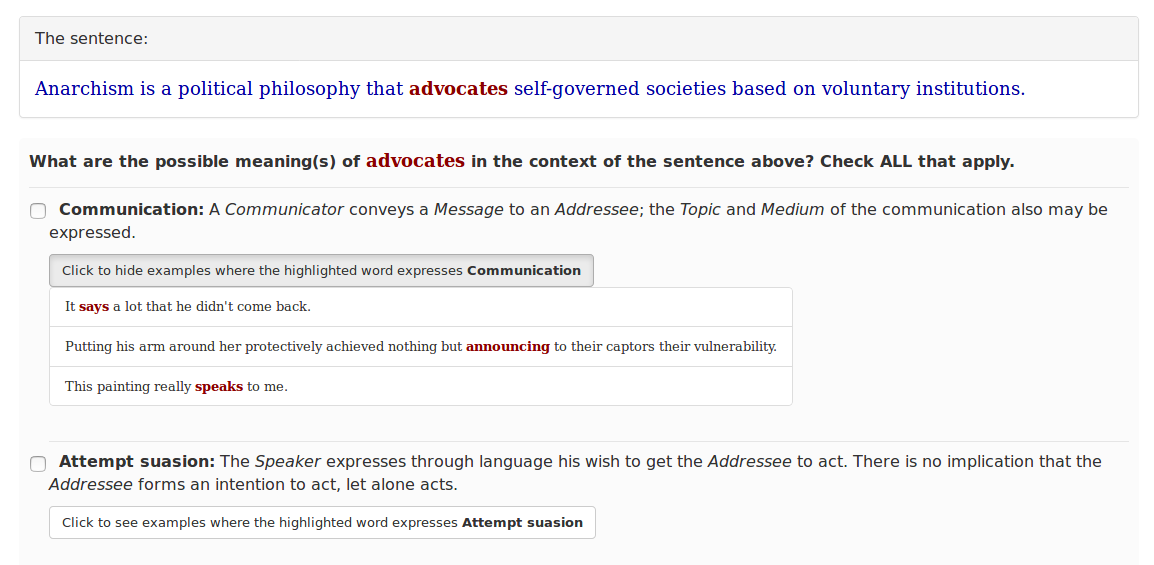
\includegraphics[width=\textwidth]{img/sent-frame.png}
\caption{Fragment of the crowdsourcing task template.}
\label{fig:ch5template}
\end{figure}


The crowdsourcing task was run on the Amazon Mechanical Turk platform\footnote{\url{https://mturk.com/}}. The task template is shown in Figure~\ref{fig:ch5template}. The workers were given a sentence with the word highlighted, and then asked to perform the multiple choice task of selecting all frames that fit the sense of the highlighted word, or that none of the frames fit. The most challenging part of the frame disambiguation task design is making sure that the crowd can understand the meaning of the frame. For each frame, we show the definition, as well as a list of sentences exemplifying the usage of the frame. These example sentences can be accessed by the workers by clicking a button next to each frame, so that the workers do not become overwhelmed with the information on the task page. In order to make sure we capture diverse worker opinions, we increased the number of annotators per sentence from 10 (the number recommended by \citet{Hong:2011:GCR:2018966.2018970}), to 15. The cost of the task varied from \$0.08 per annotation at the start of the task, in order to attract a sizable pool of workers, to \$0.06 at the end, as workers became quicker at solving the task.

\subsection{Disagreement Metrics}
\label{sec:frame-metrics}

To aggregate the results of the crowd, while also capturing inter-annotator disagreement, we use a modified version of the CrowdTruth~\cite{aroyo2014threesides} metrics. The first step is to construct the \textit{worker vectors}, which are a set of binary vectors encoding the decision of one worker for one sentence. The vector has $n+1$ components, where $n$ is the number of frames shown together with the sentence. If the worker selects a frame from the multiple-choice list, its corresponding component would be marked with `1', and `0' otherwise. The decision to pick none of the frames also corresponds to a component in the vector. Using these worker vectors, we then calculate the following disagreement metrics:

\begin{itemize}
\item \textbf{frame-sentence score (FSS):} the degree with which a frame matches the sense of the word in the sentence. It is the ratio of workers that picked the frame to all the workers that read the sentence, weighted by the worker quality (WQS).  A higher FSS should indicate that the frame is more clearly expressed in a sentence.

\item \textbf{sentence quality (SQS):} the overall worker agreement over one sentence. It is the average cosine similarity over all worker vectors for one sentence, weighted by the worker quality (WQS) and frame quality (FQS). A higher SQS should indicate a clear sentence.

% \item \textbf{frame quality (FQS):} the agreement over a frame in all sentences that it appears. Given frame $f$, $ FQS(f) = P(X$ annotates $f$ in $s | Y$ annotates $f$ in $s$), $\forall$ workers $X, Y$ and sentences $s$. $FQS$ is also weighed by the quality of the workers and the sentences.  A higher FQS should indicate a clear frame semantics.
\item \textbf{frame quality (FQS):} the agreement on a frame in all sentences that it appears. Given frame $f$, $ FQS(f) = avg(FSS(f,s) | FSS(f,s) > 0)$. $FQS$ is also weighed by the quality of the workers and the sentences.  A higher FQS should indicate a clear frame semantics.

\item \textbf{worker quality (WQS):} the overall agreement of one crowd worker with the other workers, calculated using average cosine similarity with other workers per sentence, and weighted by the sentence and frame qualities.

\end{itemize}

These definitions are mutually dependent, e.g. the definition of SQS depends on the FQS and WQS, the intuition being that low quality workers should not make sentences look bad, and low quality sentences should not make workers look bad, etc.  The mutual dependence requires an iterative  dynamic programming approach, which converged in numerous applications in fewer than 8 iterations.

\begin{table}[tb!]
\centering

\scalebox{0.8}{
\begin{tabular}{cp{8cm}cc}
\toprule
\textsc{\#} & \textsc{Sentence} & \textsc{Frame} & \textsc{FSS} \\ \toprule

\multirow{4}{*}{S1} & \multirow{4}{8cm}{Shops \textit{aimed} at the tourist market are interspersed with the more workaday ironmongers.} & \multirow{2}{*}{$aiming$} & \multirow{2}{*}{0.808} \\
& & & \\ %\cline{3-4}
& & \multirow{2}{*}{$purpose^{(*)}$} & \multirow{2}{*}{0.288} \\
& & & \\ \hline

\multirow{2}{*}{S2} & \multirow{2}{8cm}{The major \textit{changes} were not to daily tasks and routines , but to the political power base.} & $cause\ change$ & 0.804 \\  %\cline{3-4}
& & $undergo\ change^{(*)}$ & 0.305 \\ \hline

\multirow{2}{*}{S3} & \multirow{2}{8cm}{This \textit{investigation} has been stymied stopped, obstructions thrown up every step of the way.} & $criminal\ investigation$ & 0.898 \\  %\cline{3-4}
& & $scrutiny^{(*)}$ & 0.377 \\ \hline

\multirow{2}{*}{S4} & \multirow{2}{8cm}{Does supersizing \textit{cause} obesity?} & $cause\ to\ start$ & 0.804 \\  %\cline{3-4}
& & $causation^{(*)}$ & 0.608 \\ \hline

\multirow{4}{*}{S5} & \multirow{4}{8cm}{The loud, raucous Jamaican English dialect and the \textit{waving} hands reflect the joy with which social relations are conducted here.} & \multirow{2}{*}{$body\ movement$} & \multirow{2}{*}{0.861} \\
& & & \\ %\cline{3-4}
& & \multirow{2}{*}{$gesture^{(*)}$} & \multirow{2}{*}{0.463} \\
& & & \\ \hline

\multirow{2}{*}{S6} & \multirow{2}{8cm}{The Intifada \textit{heralded} the rise of the Muslim fundamentalism.} & $heralding$ & 0.777 \\  %\cline{3-4}
& & $omen^{(*)}$ & 0.227 \\ \hline

\multirow{2}{*}{S7} & \multirow{2}{8cm}{Fish (heads discreetly \textit{wrapped} in paper) are still hung out to dry in the sun.} & $adorning$ & 0.31 \\  %\cline{3-4}
& & $filling^{(*)}$ & 0.278 \\ %\hline
\bottomrule
\end{tabular}
}

\caption{Example sentence-word pairs where the top crowd frame choice is different than the expert. The targeted word appears in italics font in the sentence. The frame picked by the expert is marked with $^{(*)}$.}
\label{tab:disagr}
\end{table}

\section{Crowd vs. Experts}
\label{sec:frame-crowd-exp}

To evaluate the quality of the crowd annotations, we iterate through different values of thresholds in the FSS to classify a frame-sentence pair as either positive or negative, then compare the results with the annotations of the FrameNet experts. The results for both the micro (i.e. each frame-sentence pair is counted as either true positive, false positive etc. and used in the calculation of the F1 and accuracy) and macro (the F1 and accuracy are calculated for each sentence and each frame, and then averaged into the final values) scores are presented in Figures~\ref{fig:sent_f1} \&~\ref{fig:sent_acc}.

\begin{figure}[tbh!]
\centering
\begin{subfigure}{.5\textwidth}
\centering
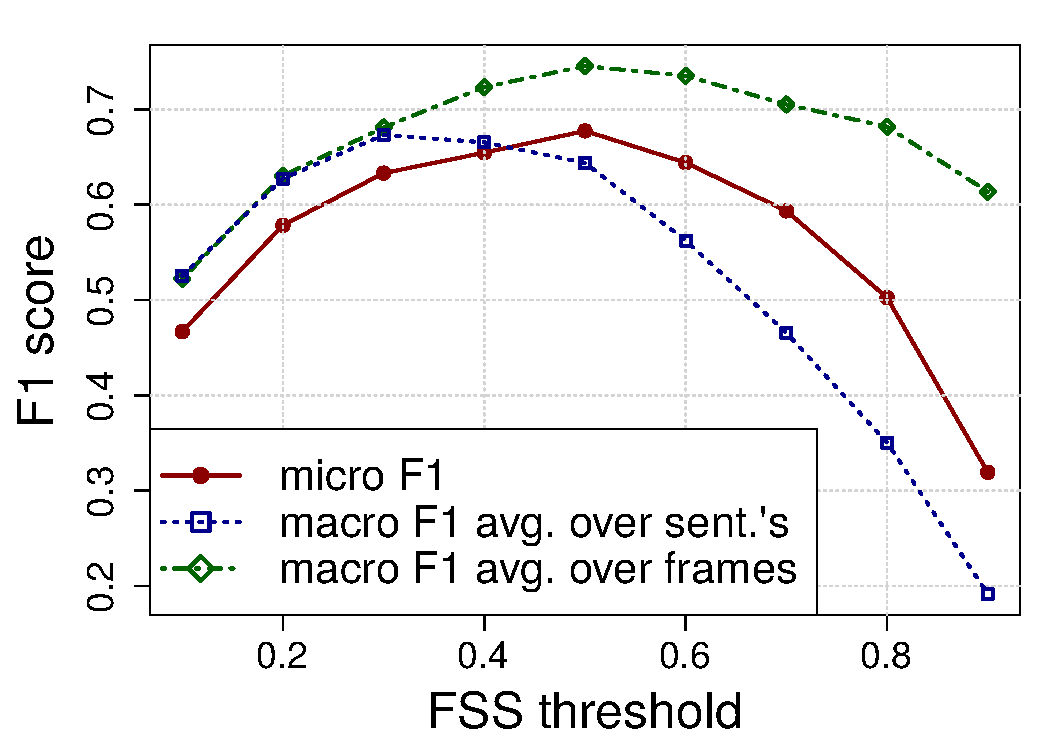
\includegraphics[width=\linewidth]{img/sent_f1_micro_macro.pdf}
\caption{F1 score}
\label{fig:sent_f1}
\end{subfigure}%
\begin{subfigure}{.5\textwidth}
\centering
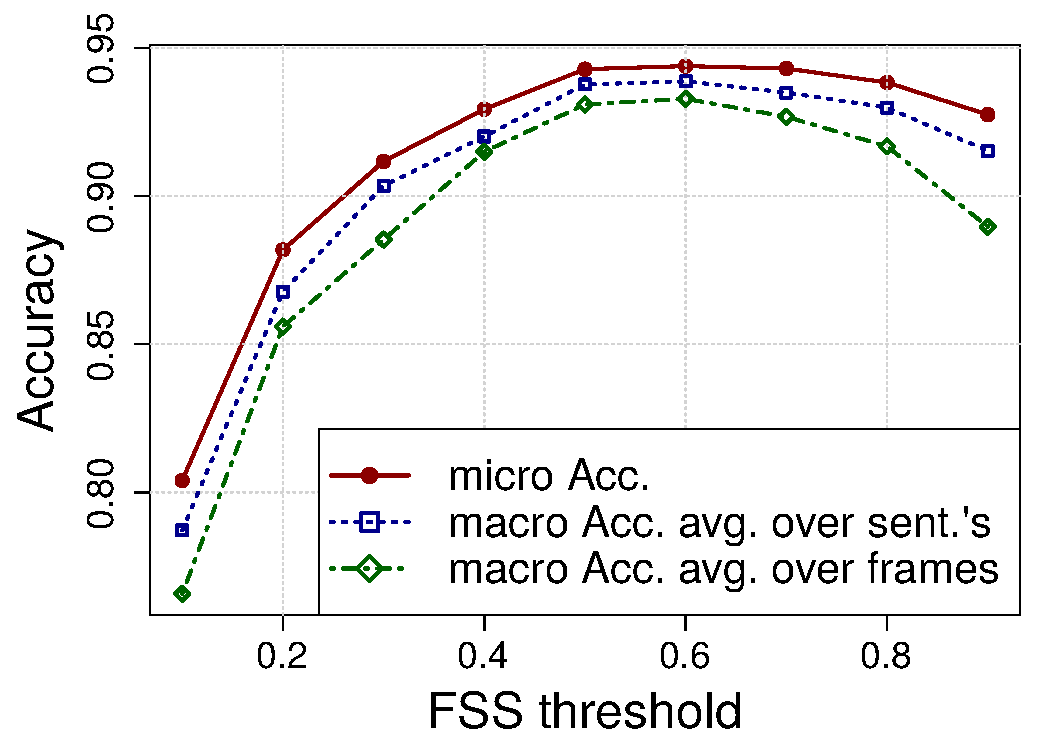
\includegraphics[width=\linewidth]{img/sent_acc_micro_macro.pdf}
\caption{Accuracy}
\label{fig:sent_acc}
\end{subfigure}
\caption{Crowd evaluation results, using expert annotation as correct.}
\end{figure}

At the best FSS threshold, the accuracy scores are comparable to those presented by \citet{Hong:2011:GCR:2018966.2018970}, who report an average accuracy of 0.928, although on a different dataset. However, accuracy in multi-class classification problems are unreliable as there are high numbers of true negatives. The F1 score is likely a more reliable metric of the performance of the crowd, with scores $ > 0.67 $ for all 3 versions of the F1. Finally, an ANOVA test over the paired FSS and expert decision for a frame-sentence pair resulted in the $ F-value = 4597 $ and $p < 2e^{-16} $, proving that there is a statistically significant relationship between the crowd FSS and the decision of the expert.

\begin{table}[tb!]
\centering

\scalebox{0.8}{
\begin{tabular}{cp{5.5cm}ccc}
\toprule
\textsc{\#} & \textsc{Sentence} & \textsc{SQS} &  \textsc{Frame} & \textsc{FSS}  \\ \toprule

\multirow{5}{*}{P1} & \multirow{5}{5.5cm}{Egypt has provided no evidence demonstrating the \textit{elimination} of its biological warfare ability, which has existed since at least 1972.} & \multirow{5}{*}{0.841} & & \\
& & & $removing^{(*)}$ & 0.938 \\ %%\cline{4-5}
& & & $cause\ change$ & 0.175 \\ %%\cline{4-5}
& & & $event$ & 0.032 \\
& & & &  \\ \hline

\multirow{4}{*}{P2} & \multirow{4}{5.5cm}{First, he forbade seeking the aid of infidels when the Syrian Mujahiddin asked Saddam Hussein to \textit{overthrow} the regime of Hafiz Al-Assad in Syria.} & \multirow{4}{*}{0.669} & $change\ of\ leadership^{(*)}$ & 0.847 \\  %\cline{4-5}
& & & $removing$ & 0.539 \\ %\cline{4-5}
& & & $eventive\ cognizer\ affecting$ & 0.087 \\ %\cline{4-5}
& & & $people$ & 0.005 \\ \hline

\multirow{5}{*}{P3} & \multirow{5}{5.5cm}{Their influence helped draw a line in the desert sand between legitimate operations and mob casinos, where illegal \textit{skimming} of profits was rampant.} & \multirow{5}{*}{0.366} & $removing^{(*)}$ & 0.532 \\ %\cline{4-5}
& & & $theft$ & 0.494 \\ %\cline{4-5}
& & & $committing\ crime$ & 0.459 \\ %\cline{4-5}
& & & $misdeed$ & 0.431 \\ %\cline{4-5}
& & & $cause\ change$ & 0.273 \\ \toprule

\multirow{4}{*}{P4} & \multirow{4}{5.5cm}{The above mentioned protection \textit{procedures} are only for observation purposes, while patrols check the fences, the barriers, and the towers.} & \multirow{4}{*}{0.786} & \multirow{2}{*}{$means^{(*)}$} & \multirow{2}{*}{0.889} \\
& & & &  \\ %\cline{4-5}
& & & \multirow{2}{*}{$being\ employed$} & \multirow{2}{*}{0.11} \\
& & & & \\ \hline

\multirow{4}{*}{P5} & \multirow{4}{5.5cm}{We've expanded Goodwill's proven \textit{methods} to towns and neighborhoods where they are needed most.} & \multirow{4}{*}{0.364} & $means^{(*)}$ & 0.601 \\ %\cline{4-5}
& & & $expertise$ & 0.342 \\ %\cline{4-5}
& & & $domain$ & 0.173 \\ %\cline{4-5}
& & & $fields$ & 0.131 \\ \hline

\multirow{4}{*}{P6} & \multirow{4}{5.5cm}{The latest \textit{approach} is perhaps the best of the post-mob era : the comprehensive resort.} & \multirow{4}{*}{0.208} & $means^{(*)}$ & 0.457 \\ %\cline{4-5}
& & & $conduct$ & 0.225 \\ %\cline{4-5}
& & & $path\ traveled$ & 0.159 \\ %\cline{4-5}
& & & $communication$ & 0.121 \\ \toprule

\multirow{6}{*}{P7} & \multirow{6}{5.5cm}{Prime Minister Ariel Sharon of Israel \textit{urged} President Bush to step up pressure on Iran to give up all elements of its nuclear program.} & \multirow{6}{*}{0.528} & & \\
& & & $attempt\ suasion^{(*)}$ & 0.81 \\ %\cline{4-5}
& & & $request$ & 0.387 \\ %\cline{4-5}
& & & $communication$ & 0.337 \\ %\cline{4-5}
& & & $cause\ to\ start$ & 0.115 \\
& & & & \\ \hline

\multirow{4}{*}{P8} & \multirow{4}{5.5cm}{The security team should \textit{urge} everyone to take precautions and guard their homes tightly.} & \multirow{4}{*}{0.358} & $attempt\ suasion^{(*)}$ & 0.605 \\ %\cline{4-5}
& & & $request$ & 0.321 \\ %\cline{4-5}
& & & $cause\ to\ start$ & 0.256 \\ %\cline{4-5}
& & & $communication$ & 0.213 \\ \hline

\multirow{4}{*}{P9} & \multirow{4}{5.5cm}{The security team should publish a periodic bulletin and distribute to all residents, \textit{advising} them how to safely store gaz and logs.} & \multirow{4}{*}{0.386} & $attempt\ suasion^{(*)}$ & 0.576 \\ %\cline{4-5}
& & & $communication$ & 0.567 \\ %\cline{4-5}
& & & $expertise$ & 0.167 \\ %\cline{4-5}
& & & $request$ & 0.156 \\ %\hline
\bottomrule
\end{tabular}
}
\caption{Different FSS values for the frames $removing$ (P1, P2, P3), $means$ (P4, P5, P6), $attempt\ suasion$ (P7, P8, P9). The targeted word appears in italics font in the sentence. The frame picked by the expert is marked with $^{(*)}$.}
\label{tab:fss_ex}
\end{table}

While the majority of expert choices have high FSS scores, there are some exceptions. We observed 3 different causes for this disagreement, which are exemplified in Table~\ref{tab:disagr}:

\begin{enumerate}

\item The crowd \textit{misunderstood the frame definition}. For instance, in $S1$, the crowd mistook the $aiming$ frame to mean purpose, instead of the more literal meaning of the frame of adjusting an instrument to reach a target. In $S2$, the crowd correctly identifies a causal sense, but the correct interpretation is a passive change (\textit{changes [...] to the political power}) instead of the active change (i.e. a subject is doing the changing) that is picked by the crowd.

\item The \textit{information in the sentence is incomplete} to identify the correct frame. $S3$ does not express whether the investigation is criminal in nature, although that is a possible interpretation. This represents a limitation in the design of the crowdsourcing task -- in some versions of the expert task, annotators had the full context of the document available when performing the annotations. This could be fixed or reduced by providing the sentence before and after, without overloading the workers.

\item The crowd offers a \textit{legitimate alternative interpretation} of what the correct frame should be. In $S5$ the crowd picks the more general frame $body\ movement$ for \textit{waving}, while in $S4$ and $S6$, the crowd picks more specific interpretations than the expert ($cause\ to\ start$ for the \textit{obesity} effect instead of the broader sense of $causation$ in $S4$, and $heralding$ instead of $omen$ for the word \textit{heralding} in $S6$). $S7$ shows an example where the expert made a mistake, as $filling$ refers to the action of covering an area with something, whereas $adorning$ refers to the passive act of being covered.

\end{enumerate}


\section{Capturing Ambiguity}
\label{sec:frame-ambig}

The cases where the experts and crowd disagree exemplify how difficult frame disambiguation can be when dealing with ambiguity, both in sentences and in the frame definition. Currently in the FrameNet corpus, the expert annotations lack the level of granularity necessary to differentiate between clear expressions of the frames, and more ambiguous ones. We propose the FSS metric as a method to capture the degree of ambiguity with which a frame captures a word sense in a sentence. In Table~\ref{tab:fss_ex}, we show how the FSS metric varies together with the clarity with which a frame is expressed across different sentences. We demonstrate this across 3 different frames:

\begin{itemize}

\item $removing$: $P1$ is an unambiguous expression of the frame, as reflected by the high agreement score. In $P2$, the top crowd frame as well as the expert choice frame $change\ of\ leadership$ refers to overthrowing the government, and $removing$ can be read as a generalization of this sense (i.e. removing the government by overthrowing it) -- $removing$ is a valid interpretation, but less specific, and the lower FSS seems justified. $P3$ is an even more ambiguous case -- it is not clear whether the word \textit{skimming} refers to generally $committing\ crime$, or to the more specific crime of $theft$, and $removing$ is a generalization for the sense of $theft$, however skimming here is a common metaphor, and not the actual act of skimming. We claim the rank ordering of uses of the \textit{removing} frame here is sensible, moreover it is far more useful to capture this information than require a single discrete truth value - the third case is simply not as clear a usage of the frame as the first.  There is a certain arbitrariness to determining which of these is "truly removing" and which is not.



\begin{figure}[tbh!]
\centering
\begin{subfigure}{.5\textwidth}
\centering
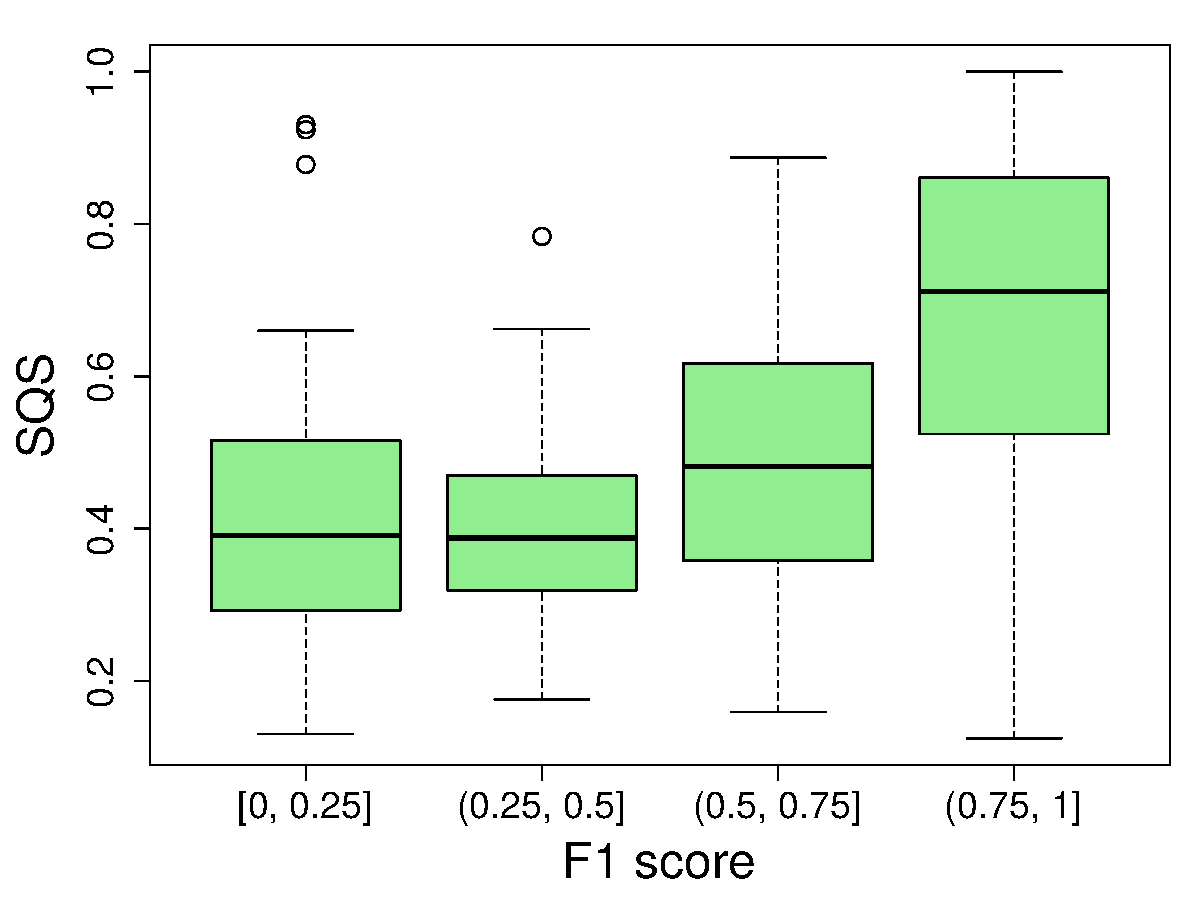
\includegraphics[width=\linewidth]{img/sqs_f1.pdf}
\caption{SQS in relation to F1 score (with \\ expert annotations as true positives), shows that in higher quality sentences, the crowd tends to agree with experts.}
\label{fig:sqs_f1}
\end{subfigure}%
\begin{subfigure}{.5\textwidth}
\centering
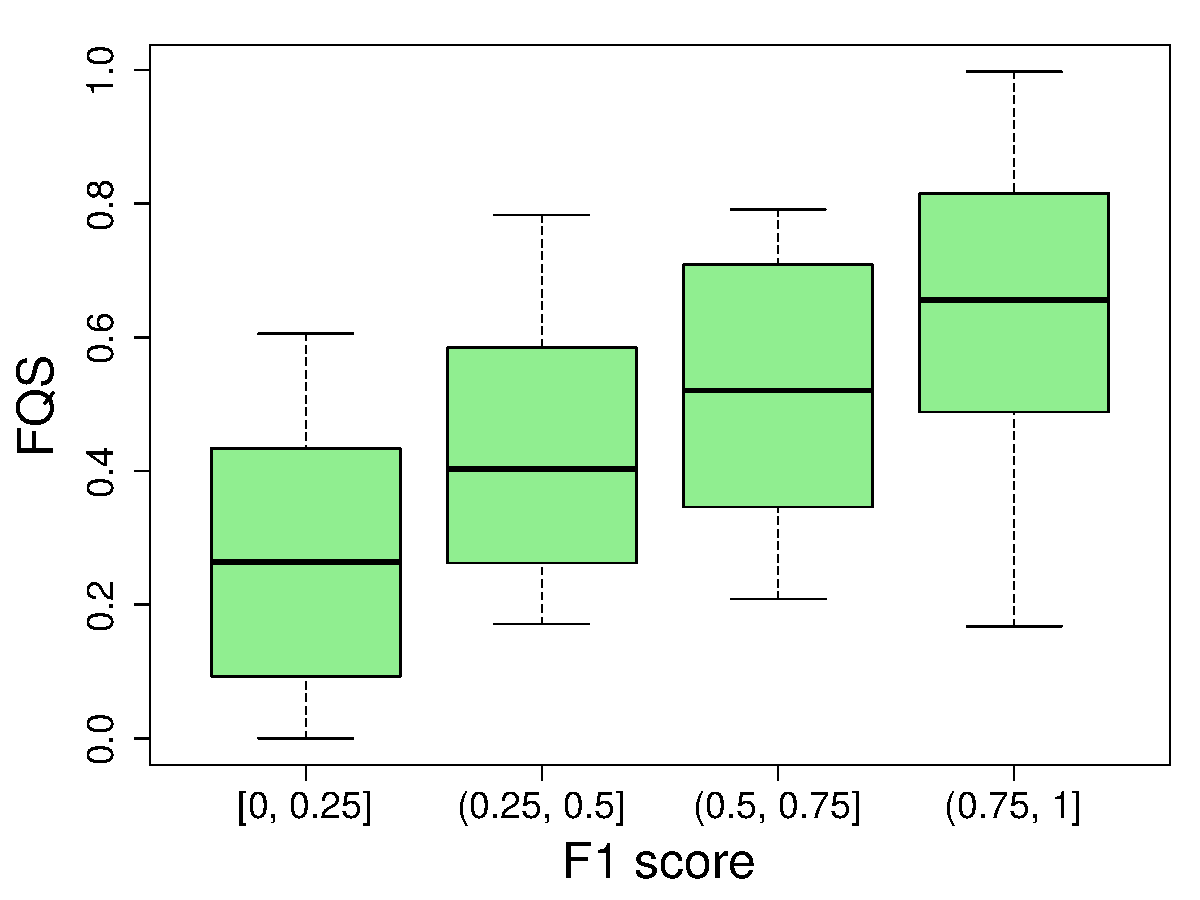
\includegraphics[width=\linewidth]{img/fqs_f1.pdf}
\caption{FQS in relation with F1 score (with expert annotations as true positives), shows that in higher quality frames, the crowd tends to agree with the experts.}
\label{fig:fqs_f1}
\end{subfigure}
\caption{SQS \& FQS evaluation.}
\end{figure}

\begin{table}[tbh!]
\centering

\scalebox{0.8}{
\begin{tabular}{cp{6cm}ccc}
\toprule
\textsc{\#} & \textsc{Sentence} & \textsc{SQS} &  \textsc{Frame} & \textsc{FSS}  \\ \toprule

\multirow{6}{*}{Q1} & \multirow{6}{6cm}{Although David bought the land for the Temple and carefully assembled its building materials, he was deemed unworthy of \textit{constructing} the Temple.} & \multirow{6}{*}{0.711} & \multirow{2}{*}{$building^{(*)}$} & \multirow{2}{*}{0.925} \\
& & & & \\  %\cline{4-5}
& & & \multirow{2}{*}{$manufacturing$} & \multirow{2}{*}{0.183} \\ 
& & & & \\ %\cline{4-5}
%& & & $cause\ to\ start$ & 0.156 \\
%& & & $coming\ up\ with$ & 0.069 \\
& & & \multirow{2}{*}{$create\ physical\ artwork$} & \multirow{2}{*}{0.056} \\
& & & & \\ \hline

\multirow{6}{*}{Q2} & \multirow{6}{6cm}{Passageways for cars and pedestrians should be designated 4- Road bumps: Six successive bumps should be \textit{constructed} at 500 meters from the location.} & \multirow{6}{*}{0.542} & \multirow{2}{*}{$building^{(*)}$} & \multirow{2}{*}{0.768} \\
& & & & \\ %\cline{4-5}
& & & \multirow{2}{*}{$manufacturing$} & \multirow{2}{*}{0.326} \\ 
& & & & \\  %\cline{4-5}
& & & \multirow{2}{*}{$create\ physical\ artwork$} & \multirow{2}{*}{0.089} \\
& & & & \\ \hline
% & & & $cause\ change$ & 0.082 \\ 
% & & & $cause\ to\ start$ & 0.082 \\ \hline

\multirow{4}{*}{Q3} & \multirow{4}{6cm}{\textit{Constructed} in wood, brick, stone, ceramic, and bronze, this is a work of extravagant beauty, uniting many ancient art forms.} & \multirow{4}{*}{0.351} & $building^{(*)}$ & 0.515 \\ %\cline{4-5}
& & & $create\ physical\ artwork$ & 0.335 \\ %\cline{4-5}
& & & $manufacturing$ & 0.237 \\
& & & & \\ \toprule
%& & & $cause\ to\ start$ & 0.072 \\ 
%& & & $opinion$ & 0.004 \\ \toprule

\multirow{4}{*}{Q4} & \multirow{4}{6cm}{U.S. Congressman Tony Hall arrived here Sunday evening, \textit{becoming} the first U.S. lawmaker to visit Iraq since the 1991 Gulf War.} & \multirow{4}{*}{0.901} & $becoming^{(*)}$ & 0.995 \\ %\cline{4-5}
& & & $cause\ change$ & 0.24 \\ %\cline{4-5}
& & & $undergo\ change$ & 0.212 \\
& & & & \\ \hline

\multirow{4}{*}{Q5} & \multirow{4}{6cm}{Cheung Chau \textit{becomes} the center of Hong Kong life once a year, usually in May , during the Bun Festival, a folklore extravaganza.} & \multirow{4}{*}{0.562} & $becoming^{(*)}$ & 0.783 \\ %\cline{4-5}
& & & $undergo\ change$ & 0.783 \\  %\cline{4-5}
& & & $cause\ change$ & 0.402 \\
& & & & \\ \toprule

\multirow{2}{*}{Q6} & \multirow{2}{6cm}{Are there any \textit{efforts} to bring back small investors?} & \multirow{2}{*}{0.811} & $attempt^{(*)}$ & 0.926 \\ %\cline{4-5}
& & & $commitment$ & 0.178 \\ \hline

\multirow{2}{*}{Q7} & \multirow{2}{6cm}{At AOL there was a conscious \textit{effort} to develop other ``characters,'' for lack of a better word.} & \multirow{2}{*}{0.588} &  $attempt^{(*)}$ & 0.739 \\ %\cline{4-5}
& & & $commitment$ & 0.468 \\
& & & & \\ %\hline 
\bottomrule


\end{tabular}
}
\caption{Sentence Quality Score Examples. The targeted word appears in italics font in the sentence. The frame picked by the expert is marked with $^{(*)}$.}
\label{tab:sqs}
\end{table}

\item $means$: This frame refers to the means used by an agent to achieve a purpose. While $P4$ offers an unambiguous expression of the frame, in $P5$ the means with which to achieve a goal becomes confused with the expertise and knowledge required to achieve it. In $P6$ the goal is not mentioned, therefore creating confusion about the purpose of the \textit{approach}, and whether it might refer to a way of communicating or behaving.  Again, we claim this rank ordering is more informative than requiring a discrete judgment on each case.

\item $attempt\ suasion$: This frame refers to a speaker attempting to influence the addressee to act. Sentences $P7$ to $P9$ express various degrees of persuasion, from obviously to weakly expressed. In $P7$, it is clear that the attempt at persuasion is an event that has occurred (\textit{Sharon [...] urged}). $P8$ expresses an obligation at an attempt to persuade (\textit{should urge}), whereas in $P9$ the persuasion is weaker, merely \textit{advice}.


\end{itemize}

In addition to the ranking, the method of collecting data from multiple crowd workers yields alternate interpretations, which are also quite useful.  Consider that a common motivation for collecting annotated data is to train and evaluate deep learning models, many of which produce vectors of output (frame disambiguation can be implemented as a multi-class problem).  Our methods of gathering annotations are naturally suited to multi-class objectives.

The SQS and FQS metrics can additionally be used to express the overall ambiguity in the sentence and frame, respectively. Figures~\ref{fig:sqs_f1} \&~\ref{fig:fqs_f1} show that sentences with higher SQS and frames with higher FQS also have higher F1 values, demonstrating that the SQS and FQS metrics can be useful in determining data quality. This result, in combination with the correlation between FSS and expert annotations, shows that when there is agreement in the crowd, then the crowd also agrees with the experts, but when there is disagreement, it may be because something is wrong: with the workers, the sentence, or the frames.

In Table~\ref{tab:sqs}, we show some examples of how SQS captures the clarity for the sense of a word in a sentence, by taking the same word (and therefore same list of candidate frames) in different sentences:



\begin{table}[tb!]
\centering

\scalebox{0.8}{
\begin{tabular}{ccp{3.5cm}p{5.5cm}c}
\toprule
\textsc{Frame} & \textsc{FQS} & \textsc{Definition} & \textsc{Example Sentences} & \textsc{FSS} \\ \toprule


\multirow{7}{*}{$killing$} & \multirow{7}{*}{0.954} & \multirow{7}{3.5cm}{A Killer or Cause causes the death of the Victim.} &  $F1$: Older kids left homeless after a recent murder-\textit{suicide} in Indianapolis claimed Mom and Dad. & 0.8 \\ %\cline{4-5}
& & & $F2$: The incident at Mayak was the third \textit{shooting} in recent weeks involving nuclear weapons or facilities in Russia. & 0.75 \\ \hline

\multirow{9}{*}{$food$ } & \multirow{9}{*}{0.838} & \multirow{9}{3.5cm}{Words referring to items of food.} & $F3$: Lamma Island is perfect for sitting back to watch \textit{bananas} grow. & 1.0 \\ %\cline{4-5}
& & & $F4$: Along with the usual \textit{chickens}, you will see for sale snakes, dogs, and sometimes monkeys - all highly prized delicacies . & 0.838 \\ %\cline{4-5}
& & & $F5$: You can browse among antiques, flowers, \textit{herbs}, and more. & 0.503 \\ \hline

\multirow{7}{*}{$assistance$ } & \multirow{7}{*}{0.634 } & \multirow{7}{3.5cm}{A Helper benefits a Benefited party by enabling the culmination of a Goal of the Benefited party.} & $F6$: Your support \textit{helps} provide real solutions. & 0.955 \\  %\cline{4-5}
& & & $F7$: Unemployment \textit{provides} benefits that many entry-level jobs don't. & 0.467 \\  %\cline{4-5}
& & & $F8$: Your support of Goodwill will \textit{provide} job training. & 0.401 \\ \hline

\multirow{8}{*}{$purpose$ } & \multirow{8}{*}{0.63 } & \multirow{8}{3.5cm}{An Agent wants to achieve a Goal. A Means is used to allow the Agent to achieve a Goal.} & $F9$: The \textit{objective} of having kiosks is they serve as communication points between the guards & 0.94 \\ %\cline{4-5}
& & & $F10$: They are antiviral drugs \textit{designed} to shorten the flu. & 0.476 \\  %\cline{4-5}
& & & $F11$: It seems that the city produced artists of this stature by accident, even against its \textit{will}. & 0.241 \\ \hline

\multirow{7}{1cm}{$subjective$ $influence$} & \multirow{7}{*}{0.366} & \multirow{7}{3.5cm}{An Agent has influence on a Cognizer. The influence may be general, manifested in an Action as a consequence of the influence.} & $F12$: There have been changes, many of them due to economic progress, new construction, and other factors that \textit{influence} cities. & 0.54 \\ %\cline{4-5}
& & & $F13$: The Cycladic culture was \textit{influenced} by societies in the east. & 0.46 \\ %\cline{4-5}
& & & $F14$: Their complaint: the system \textit{discourages} working. & 0.364 \\ \hline

\multirow{8}{1cm}{$undergo$ $change$} & \multirow{8}{*}{0.313} & \multirow{8}{3.5cm}{An Entity changes, either in its category membership or in terms of the value of an Attribute.} & $F15$: The animosity between these two traditional enemies is beginning to \textit{diminish}. & 0.805 \\  %\cline{4-5}
 & & & $F16$: The \textit{shift} in the image of Gates has been an interesting one for me to watch. & 0.351 \\ %\cline{4-5}
& & & $F17$: The settlements of Thira and Akrotiri \textit{thrived} at this time. & 0.256 \\ %\hline
\bottomrule

\end{tabular}
}

\caption{Frame Quality Score Examples. The targeted word appears in italics font in the sentence.}
\label{tab:fqs}
\end{table}

\begin{itemize}

\item Sentences $Q1$, $Q2$ and $Q3$ all contain the word \textit{construct}, with different degrees of clarity. When the object being constructed is a building (i.e. the \textit{Temple} in $Q1$), there is no ambiguity in selecting the $building$ frame, but when the object is a \textit{road bump} ($Q2$), the sense of the building $frame$ becomes difficult to separate from $manufacturing$. In $Q3$, the object of the construction is not expressed, but the construction materials imply a precious object, therefore $building$, $manufacturing$ and $create\ physical\ artwork$ are all possible interpretations. Sentences 

\item $Q4$ and $Q5$ illustrate the variation in clarity for the word \textit{become}. While in $Q4$, the sense $becoming$ is the unambiguous choice, in $Q5$ it is difficult to choose between the frames $becoming$ and $undergo\ change$ (it is arguable that \textit{Cheung Chau} needs to undergo some form of change in order to become a center).

\item $Q6$ and $Q7$ both deal with the word \textit{effort}. In $Q7$, however, the \textit{conscious} qualifier for the word \textit{effort}, as well as the goal to \textit{develop}, implies a sustained, long-term action that can be understood as either an $attempt$ or a $commitment$ to achieve a goal. In contrast, $Q6$ expresses a short-term, concrete action (to \textit{bring}), which more closely fits the sense of the frame $attempt$.

\end{itemize}

Again, our claim is that these scores and ranking are far more sensible and informative than requiring a discrete truth decision, which seems more arbitrary as the scores decrease.

As the examples above indicate, one possible cause for sentence ambiguity is missing context information (e.g. in $Q3$). This was also one of the causes for disagreement between crowd and expert. A solution to this problem would be to expand the input text for the crowdsourcing task, to include the full paragraph, or even just one sentence before and one after the one we want the crowd to annotate.

Another reason for sentence ambiguity is frames that overlap in meaning (e.g. in $Q5$ and $Q7$). While providing more context could help with this, it is often the case that even the definitions of the frames are very close. The FQS metric is a useful indicator for these case.

Table~\ref{tab:fqs} shows varying FQS values for different frames, from very clear to ambiguous. The frame $subjective\ influence$, with an FQS of 0.366, has a low score compared to the others. From looking at the sentences, we observed that the crowd had difficulty distinguishing between this frame and $objective\ influence$. The difference between these two frames is very small -- $subjective\ influence$ means a general, vague type of influence, whose effect cannot be measured, whereas $objective\ influence$ refers to a more concrete type of influence. However, as we see from the example sentences in Table~\ref{tab:fqs}, these cases can be very difficult to separate in natural language (e.g. in $F13$ is \textit{cultural influence} subjective or objective?).

Another feature we observed was the correlation of FQS with how abstract the sense of the frame is. Frames with high FQS, such as $killing$ and $food$, tend to refer to concrete events or objects. These frames can still appear in ambiguous contexts (e.g. in $F5$, it is not clear whether \textit{herbs} classify as a type of $food$), but overall these frames refer to specific and particular senses that are unambiguous. As the value of the FQS metric goes down, the frames become more abstract. $assistance$ and $purpose$ both have example sentences where they are expressed unambiguously ($F6$ and $F9$), but their definitions are more abstract, and therefore have more room for interpretation. For instance, providing benefits (in $F7$) or expertise (in $F8$) can be regarded as a type of help, or $assistance$, even though the expert picked the more literal sense of the frame $supply$ for both of these cases. Likewise the frame $purpose$ can be understood in $F10$ as the purpose of a design (the expert picked the more literal $coming\ up\ with$), or in $F11$ as the goal of the desire/will (the expert picked $desiring$). $undergo\ change$, the frame with the lowest FQS in Table~\ref{tab:fqs} has a very broad meaning, and is a generalization of other more specific frames: $change\ position\ on\ a\ scale$ in $F16$, and $thriving$ in $F17$.

As we have seen from these examples, ambiguity in frames is connected to ambiguity in sentences. Frames with abstract or overlapping definitions are likely to appear in ambiguous sentences, and missing context from sentences is likely to result in more ambiguous scores for the frames. While workers misunderstanding the task is also a confounding factor that adds to the noise in the data, it is clear that there are many instances where inter-annotator disagreement is legitimately a by-product of ambiguity. This is an issue with the FrameNet dataset, as it does not allow for expressing the various degrees with which a sense applies to a word in a sentence, and instead relies on binary labels (i.e. the frame is expressed or not). This results in a loss of information that could impact the various natural language processing and machine learning applications that make use of this corpus, as it sets false targets for optimization -- i.e. it seems unfair to expect a model to differentiate between highly ambiguous examples, when even human annotators are having such difficulty with them.


\section{A Frame Disambiguation Corpus with Ambiguity}
\label{sec:frame-disambig-eval}

Following from the encouraging results of crowdsourcing the FrameNet corpus, we scaled up our method and collected a corpus of 5,000 sentence-word pairs. More than 1,000 of these are lexical units not part of FrameNet. To our knowledge, it is the largest corpus of this type outside of FrameNet. To perform the collection, we re-used the crowdsourcing methodology described in Section~\ref{sec:frame-crowd-setup}, using Wikipedia as a source for the sentences. This corpus was then used to perform an evaluation of several frame disambiguation models. Our proposed evaluation methodology uses evaluation metrics that leverage the multiple answers and their confidence scores, showing that even a model that always predicts the top crowd answer will not always have the best performance.


\begin{table}[tbh!]
    \centering
    \scalebox{0.8}{
    \begin{tabular}{cp{7cm}cp{5cm}}
        \hline
        \# & \textsc{Sentence} & \textbf{$SQS$} & \textsc{Frames ($FSS$)}  \\ \hline
        1 & Domestication of plants has, over the centuries \textbf{improved} disease resistance. & 0.652 & \textit{improvement or decline} (0.823), \newline \textit{cause to make progress} (0.683) \\
        2 & He is the 5th of 8 male players in history to \textbf{achieve} this. & 0.626 & \textit{accomplishment} (0.764), \newline \textit{successful action} (0.709) \\
        3 & Albertus Magnus, a Dominican monk, \textbf{commented} on the operations and theories of alchemical authorities. & 0.511 & \textit{communication} (0.522), \newline \textit{statement} (0.703) \\
        4 & He \textbf{slices} at Hector's armor, throwing him off guard and spinning him around. & 0.319 & \textit{part piece} (0.499), \textit{cause harm} (0.4), \textit{cutting} (0.394), \textit{attack} (0.254), \textit{hit target} (0.227) \\
        5 & Another 46 steps \textbf{remain} to climb in order to reach the top, the ``terrasse'', from where one can enjoy a panoramic view of Paris. & 0.308 & \textit{left to do} (0.497), \textit{remainder} (0.478), \textit{state continue} (0.319), \textit{existence} (0.155) \\
        6 & Borzoi males frequently \textbf{weigh} more. & 0.283 & \textit{assessing} (0.421), \textit{dimension} (0.402), \newline \textit{importance} (0.128) \\ 
        7 & The dance includes bending and \textbf{straightening} of the knee giving it a touch of Cuban motion. & 0.24 & \textit{reshaping} (0.495), \textit{arranging} (0.356), \textit{body movement} (0.298), \textit{cause motion} (0.249) \\ 
        \hline
    \end{tabular}
    }
    \caption{Example sentences with disagreement over the frame annotations (candidate word in bold).}
    \label{tab:examples}
\end{table}

\subsection{Ambiguity in the Corpus}

An analysis of the corpus found many examples of inter-annotator disagreement, of which a few examples are shown in Table~\ref{tab:examples}. For 720 sentences, a majority of the workers picked at least 2 frames (examples 1-3 in Tab.\ref{tab:examples}). And for 1,514 sentences, no one frame has been picked by a majority of the workers (examples 4-7 in Tab.\ref{tab:examples}). Disagreement is also more prominent in the sentences where the lexical unit is not a part of FrameNet (Fig.\ref{fig:sqs_histo}).

The disagreement comes from a variety of causes: a parent-child relation between the frames (\textit{statement} and \textit{communication} in \#3), an overlap in the definition of the frames (\textit{accomplishment} and \textit{successful action} in \#2), the meaning of the word is expressed by a composition of frames (in \#7, ``straightening of the knee'' is a combination of \textit{reshaping} the form of the knee, \textit{arranging} the knee in the right position, and \textit{body movement}), and combinations of all of these reasons (in \#4, ``slices'' is a combination of \textit{part piece} and \textit{cause harm}, and the other frames are their children). More example sentences for each type of disagreement are available in the appendix. The sentences themselves are not difficult to understand, and it can be argued that all of them have one frame that applies the best for the word. The goal of this corpus is to show that next to this best frame for the word, there are other frames that apply to a lesser degree, or capture a different part of the meaning. When evaluating a model for frame disambiguation, it seems unfair to penalize misclassifications of frames that still apply to the word, but with less clarity, in the same way we would penalize a frame that captures a wrong meaning. Also, we argue that models should take into account that annotators do not agree over some examples, and treat them differently than clear expressions of frames. Disagreement can also be caused by worker mistakes (in \#6, \textit{dimension} refers to the size of the object, not the act of measuring the size). While we try to mitigate for this by weighing confidence scores with the worker quality, the mistakes still appear in the corpus. This type of disagreement could be useful in future work to identify examples that workers need to be trained on.

\begin{figure}[htb!]
\begin{subfigure}{.5\textwidth}
\centering
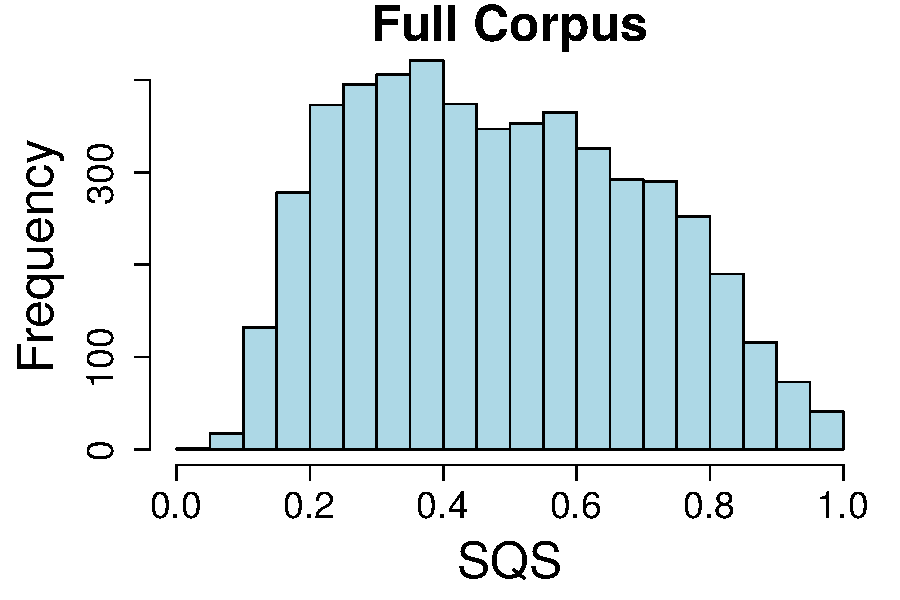
\includegraphics[width=\linewidth]{img/sqs_full.pdf}
\end{subfigure}%
\begin{subfigure}{.5\textwidth}
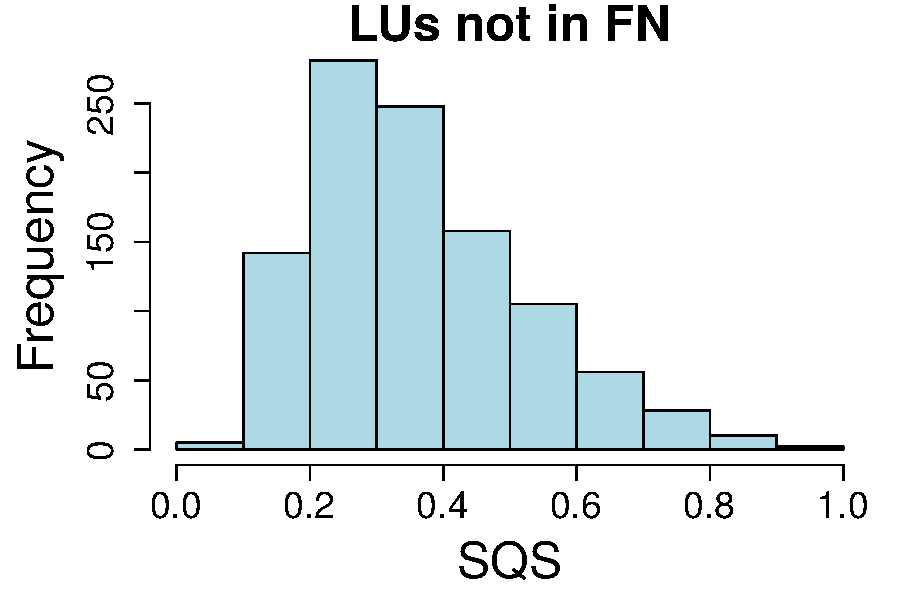
\includegraphics[width=\linewidth]{img/sqs_notfn.pdf}
\end{subfigure}
\caption{Histogram of $SQS$ values - the quality scores in sentences where the lexical unit is not in FrameNet skew lower.}
\label{fig:sqs_histo}
\end{figure}

\subsection{Systems Tested}

As an example usage of our corpus, we used it to evaluate these frame disambiguation models:

\begin{enumerate}
    \item \textbf{OS:} The Open-Sesame~\cite{swayamdipta:17} classifier, pre-trained on the FrameNet corpus (release 1.7). Given a word-sentence pair, OS uses a BiLSTM model with a softmax final layer to predict a single frame for the word. If the lexical unit is not in FrameNet, it cannot make a prediction. %OS is a BiLSTM model that uses as features the embeddings of the word type and part-of-speech, with a rectified linear unit (Relexical unit) final layer. The frame classification is performed by picking the scores from the Relexical unit layer for each candidate frame associated with the lexical unit in FrameNet, and passing them through a softmax layer to pick the top-scoring frame. Because of this, OS cannot find frames for lexical units not in FrameNet.
    
    \item \textbf{OS+:} We modified the OS classifier to perform multi-label classification. To calculate the confidence score for candidate frame $f$, we removed the softmax layer and passed the output of the BiLSTM model $\nu(f)$ through the following transformation: $c(f) = [1 + tanh \ \nu(f)] / 2$. This gave a score $c(f) \in [0,1]$ expressing the confidence that frame $f$ is expressed in the sentence.
    
    \item \textbf{FS:} Framester includes a  tool for rule-based multi-class multi-label frame disambiguation~\cite{gangemi2016framester}. While for the dataset pre-processing (Sec.~\ref{sec:frame-crowd-setup}) we considered the frames for all synsets a word is part of, FS performs an additional word-sense disambiguation step %~\cite{moro2014entity}
    to return a more precise list of frames. We used the tool with \textit{profile T} as it was shown to have the overall better performance. FS can only predict FrameNet frames from the 1.5 release, which is missing 202 frames from version 1.7. % (We expect by publication that FS will have been updated to 1.7)  As compared to our method for collecting the candidate frames~\ref{sec:corpus}, the FS tool is more precise -- it returns only the frames associated with its most likely synset, whereas we considered the frames for all synsets associated with the word. In this experiment we used \textit{profile T} of the FS tool, with the highest number of mappings, as it was shown to have the overall better performance and highest recall~\cite{gangemi2016framester}. FS is at a disadvantage compared to the other baselines, as it can only produce FrameNet frames from the 1.5 release (the latest version has an additional 202 frames). FS performs word-sense disambiguation using Babelfy~\cite{moro2014entity} to identify the WordNet~\cite{miller1995wordnet} synset associated with the word, then selects the frames through filtering over a set of manually-curated semantic mappings between the WordNet and FrameNet. 
\end{enumerate}

While OS+ produces confidence scores, the other methods produce binary labels for each frame-sentence pair. These models do not have state-of-the-art performance~\cite{hermann2014semantic,fitzgerald2015semantic}, we picked them because they were accessible and allowed testing on a novel corpus. Finally, we evaluate the quality of the \textbf{TC} corpus, containing only the top frame picked by the crowd for every sentence. This test shows what is the best possible performance over our corpus that can be expected from a system such as OS that selects a single frame per sentence. %While \textbf{OS+} produces confidence scores for each frame, the other methods produce binary labels for each frame-sentence pair. 

\subsection{Evaluation Metrics \& Results}

Instead of traditional evaluation metrics that require binary labels, we propose an evaluation methodology that is able to consider multiple candidate frames for each sentence and their quality scores. We use \textit{Kendall's $\uptau$} list ranking coefficient~\cite{kendall1938new} and \textit{cosine similarity} to calculate the distance between the list of frames produced by the crowd labeled with the $FSS$, and the frames predicted by the baselines in each sentence. Whereas Kendall's $\uptau$ only accounts for the ranking of the $FSS$ for each frame, cosine similarity uses the actual $FSS$ values in the calculation of the similarity. Both metrics compute a score per sentence (Kendall's $\uptau \in [-1,1]$, and cosine similarity $\in [0,1]$). This is similar to the method used in~\cite{dumitrache2015b}.  Using these metrics, we produce two aggregate statistics over our test corpus: (1) the area-under-curve ($AUC$) for each metric, normalized by the corpus size, and (2) the $SQS$-weighted average of each metric ($w-avg$), which also accounts for the ambiguity of the sentence as expressed by the $SQS$. We evaluate on two versions of the corpus: (1) the restricted set (\textsc{R-Set}) of 4,000 sentences with lexical units from the FrameNet corpus, and (2) the full set (\textsc{F-Set}) of 5,000 sentences.

\begin{figure}[t!]
\begin{subfigure}{.5\textwidth}
\centering
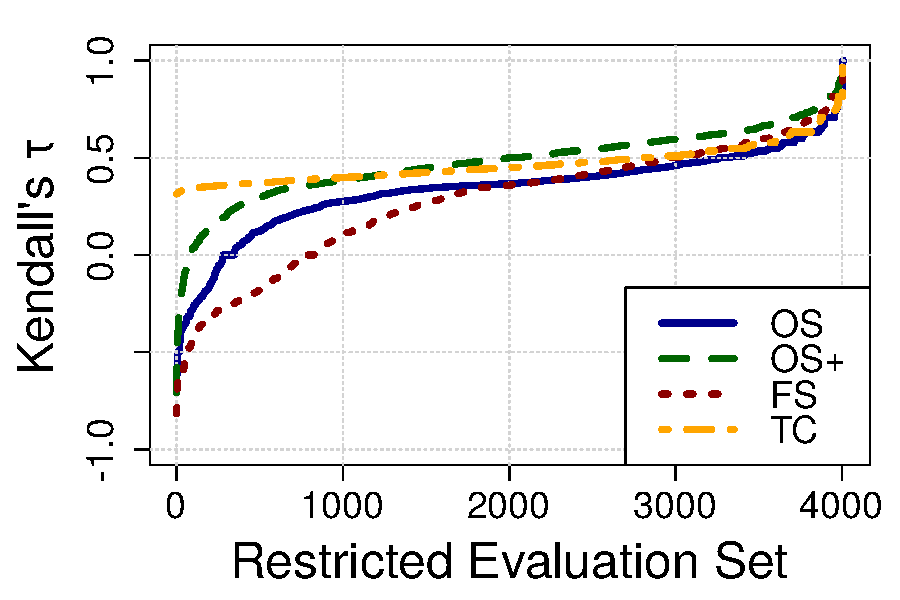
\includegraphics[width=\linewidth]{img/kendall_tau_restricted.pdf}
\end{subfigure}%
\begin{subfigure}{.5\textwidth}
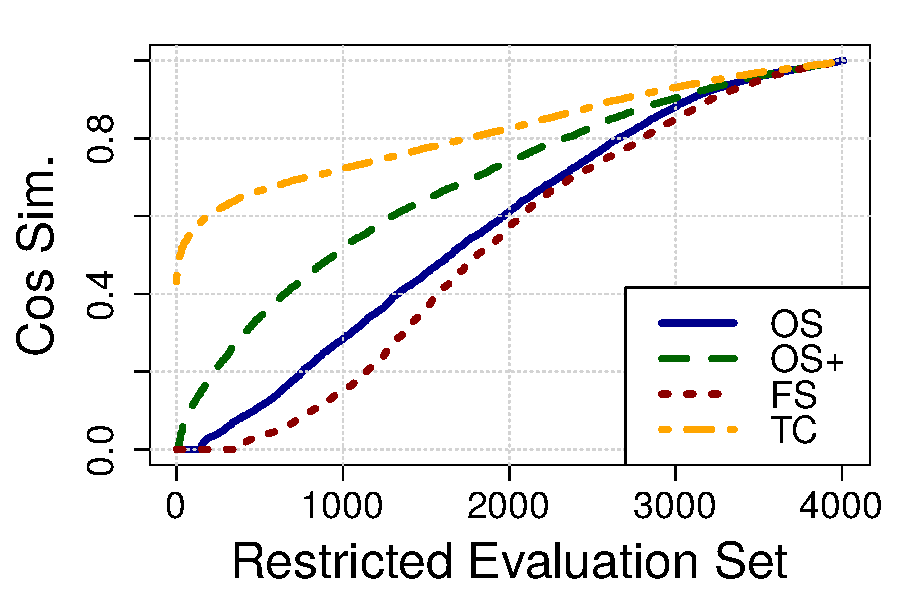
\includegraphics[width=\linewidth]{img/cos_sim_restricted.pdf}
\end{subfigure}
\begin{subfigure}{.5\textwidth}
\centering
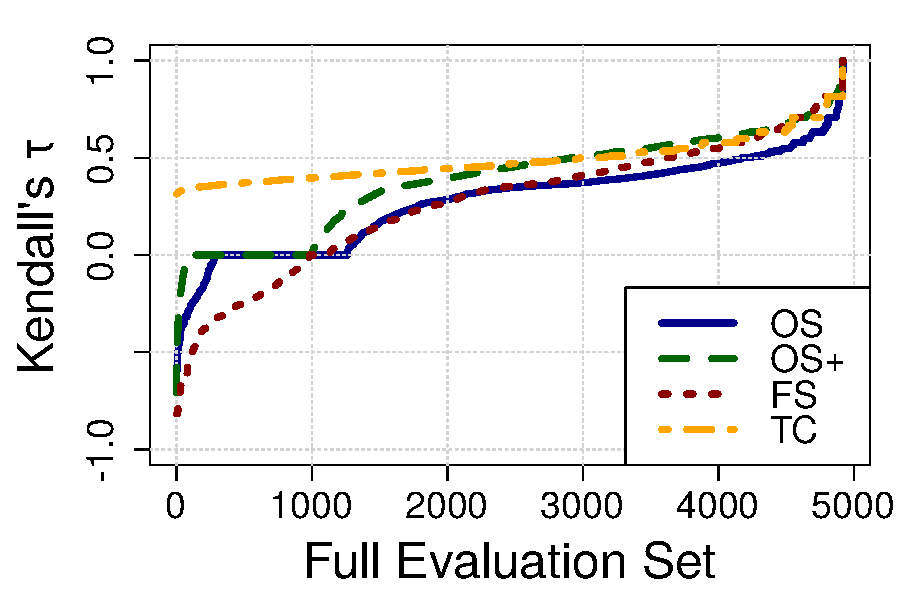
\includegraphics[width=\linewidth]{img/kendall_tau_full.pdf}
\end{subfigure}%
\begin{subfigure}{.5\textwidth}
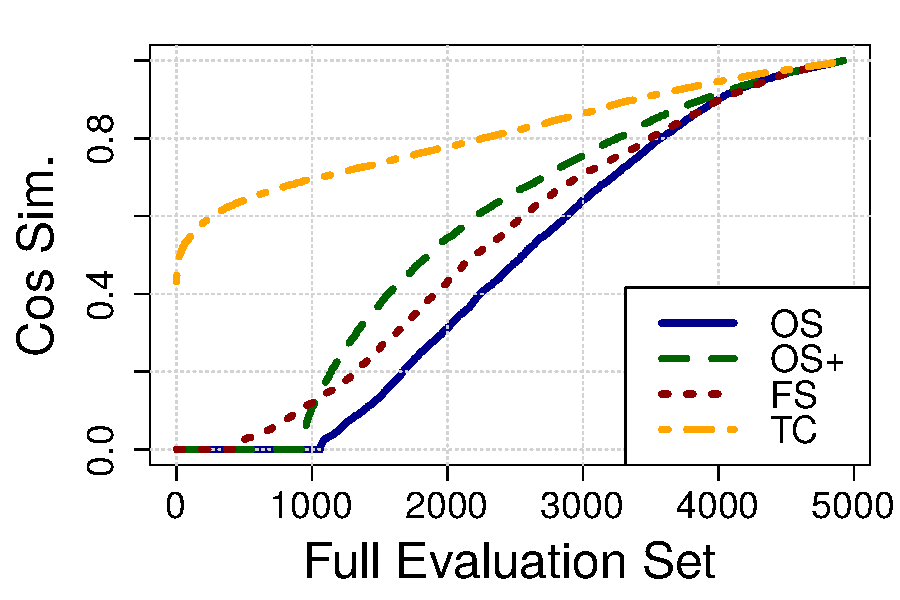
\includegraphics[width=\linewidth]{img/cos_sim_full.pdf}
\end{subfigure}
\setlength{\abovecaptionskip}{-0.0005pt}
\caption{Baselines evaluation results.}
\label{fig:eval}
\end{figure}

%\subsection{Results}

\begin{table}[t!]
    \centering
    \scalebox{0.8}{
    \begin{tabular}{cc|ccc|c}
         \hline
        %  \textbf{\textsc{Test Set}} & \textbf{\textsc{Eval. Metric}} & \textbf{OS} & \textbf{OS+}  & \textbf{FS} \\ \hline
          & \textsc{Eval. Metric} & \textbf{OS} & \textbf{OS+}  & \textbf{FS} & \textbf{TC} \\ \hline
                      & Kendall's $\uptau$  AUC & 0.339 & \textbf{0.477} & 0.279 & 0.466 \\
         \textsc{R-}  & Kendall's $\uptau$ w-avg & 0.362 & \textbf{0.497} & 0.3 & 0.48 \\
         \textsc{Set} & Cos Sim AUC & 0.57 & \textbf{0.685} & 0.518 & 0.818 \\ 
                      & Cos Sim w-avg & 0.608 & \textbf{0.717} & 0.545 & 0.854 \\ \hline
         
                     & Kendall's $\uptau$ AUC & 0.269 & \textbf{0.379} & 0.253 & 0.491 \\
         \textsc{F-} & Kendall's $\uptau$ w-avg & 0.307 & \textbf{0.421} & 0.284 & 0.501 \\
         \textsc{Set} & Cos Sim AUC & 0.453 & \textbf{0.544} & 0.511 & 0.810 \\
                      & Cos Sim w-avg & 0.515 & \textbf{0.607} & 0.539 & 0.849 \\ \hline
    \end{tabular}
    }
    \caption{Aggregated evaluation results.}
    \label{tab:results}
\end{table}

The results (Figure~\ref{fig:eval} \& Table~\ref{tab:results}) show that, even taking into account sentences with lexical units not in FrameNet for which OS+ cannot disambiguate, \textbf{the OS+ model performs best, likely because of its ability to emit predictions for the multiple frames that can apply to the same word}. FS performs the worst out of all models on \textsc{R-Set}, because it cannot find newly added frames from the latest FrameNet release, but improves on the \textsc{F-Set} (FS can find candidate frames for lexical units not in FrameNet). The scores on the \textsc{F-Set} were lower for all baselines, suggesting that \textbf{sentences with lexical units not in FrameNet are more difficult to classify} -- this could be because FrameNet is missing frames that can express the full meaning of these lexical units. TC has a good performance, but is far from being unbeatable -- when measuring Kendall's $\uptau$ over the \textsc{R-Set}, OS+ performs better than TC.



\section{Conclusion}

In this chapter, we explored how \emph{inter-annotator disagreement can be used as an indicator for language ambiguity} for the task of FrameNet frame disambiguation. To achieve this, we employed the CrowdTruth~\cite{aroyo2014threesides} method, using multiple workers per sentence in order to capture and interpret inter-annotator disagreement. We modified CrowdTruth metrics in order to capture frame-sentence agreement (FSS), sentence quality (SQS) and frame quality (FQS). We performed an experiment over a set of 433 sentences annotated with frames from FrameNet corpus, and showed that the aggregated crowd annotations achieve an F1 score greater than 0.67 compared to expert linguists, and an accuracy that is comparable to the state of the art~\cite{Hong:2011:GCR:2018966.2018970}. Afterwards, we scaled up the methodology to collect a frame disambiguation resource over 5,000 sentence-word pairs from Wikipedia, out of which 1,000 have lexical units that are new to FrameNet. This is the largest corpus of this type outside of FrameNet.

We showed cases where the crowd annotation is correct even though the expert is in disagreement, arguing for the need to have multiple annotators per sentence. Most importantly, we examined the cases in which crowd workers could not agree. We found that disagreement is caused by one or more of the following: workers misunderstanding the task, missing context from the sentences, frames with overlapping or abstract definitions. The results show a clear link between inter-annotator disagreement and ambiguity, either in the sentence, frame, or the task itself. We argue that collapsing such cases to a single, discrete truth value (i.e. correct or incorrect) is inappropriate, creating brittle, incomplete datasets, and therefore arbitrary targets for machine learning.  We further argued that ranking examples by a score is informative, and that the crowd offers alternate interpretations that are often sensible.

Finally, we proposed an evaluation method that uses the scores for multiple frames, and is thus able to differentiate between frames that still apply to the word, but with less clarity, and frames that capture the wrong meaning. Our goal was to build a resource that recognizes different levels of ambiguity in the expression of the frames in the text, and allows a more fair evaluation of performance of frame disambiguation systems.

\section*{Acknowledgments}

We would like to thank Luigi Asprino, Valentina Presutti and Aldo Gangemi for their assistance with using the Framester corpus, as well as their advice in better understanding the task of frame disambiguation. We would also like to thank the anonymous crowd workers for their contributions to our crowdsourcing tasks.

\section{Appendix: Ambiguous Dataset Examples}

\begin{table}[thb!]
    \centering
    \scalebox{0.75}{
    \begin{tabular}{cp{7cm}cp{5cm}}
        \hline
        \# & \textsc{Sentence} & \textbf{$SQS$} & \textsc{Frames ($FSS$)}  \\ \hline
        1 & These Articles have historically shaped and \textbf{continue} to direct the ethos of the Communion. & 0.795 & \textit{activity ongoing} (0.862) \newline \textit{process continue} (0.86) \\
        2 & ``A Modest Proposal'' is \textbf{included} in many literature programs as an example of early modern western satire. & 0.771 & \textit{inclusion} (0.89) \newline \textit{cause to be included} (0.813) \\ 
        3 & The states often \textbf{failed} to meet these requests in full, leaving both Congress and the Continental Army chronically short of money. & 0.628 & \textit{endeavor failure} (0.826) \newline \textit{success or failure} (0.8) \\
        4 & This is a chart of trend of nominal gross domestic product of Angola at market prices \textbf{using} International Monetary Fund data. & 0.598 & \textit{using resource} (0.831) \newline \textit{using} (0.554) \newline \textit{tool purpose} (0.336) \\
        5 & The Asian tigers have now all \textbf{received} developed country status, having the highest GDP per capita in Asia. & 0.504 & \textit{receiving} (0.751) \newline \textit{getting} (0.556) \\
        6 & MasterCard has released Global Destination Cities Index 2013 with 10 of 20 are \textbf{dominated} by Asia and Pacific Region Cities. & 0.467 & \textit{dominate situation} (0.638) \newline \textit{dominate competitor} (0.579) \newline \textit{being in control} (0.327) \\ 
        \hline
    \end{tabular}
    }
    \caption{Ambiguity because of parent-child relation between frames.}
    \label{tab:sub_super}
\end{table}



\begin{table}[thb!]
    \centering
    \scalebox{0.75}{
    \begin{tabular}{cp{7cm}cp{5cm}}
        \hline
        \# & \textsc{Sentence} & \textbf{$SQS$} & \textsc{Frames ($FSS$)}  \\ \hline
        1 & Kournikova then \textbf{withdrew} from several events due to continuing problems with her left foot and did not return until Leipzig. & 0.725 & \textit{withdraw from participation} (0.955), \textit{removing} (0.61) \\
        2 & Some aikido organizations use belts to \textbf{distinguish} practitioners' grades. & 0.68 & \textit{differentiation} (0.867) \newline \textit{distinctiveness} (0.703) \\
        3 & Since then, it has focused on \textbf{improving} relationships with Western countries, cultivating links with other Portuguese-speaking countries, and asserting its own national interests in Central Africa. & 0.654 & \textit{improvement or decline} (0.787) \newline \textit{cause to make progress} (0.732) \\ %  \newline \textit{progression} (0.386)
        4 & To \textbf{emphasize} the validity of the Levites' claim to the offerings and tithes of the Israelites, Moses collected a rod from the leaders of each tribe in Israel and laid the twelve rods over night in the tent of meeting. & 0.65 & \textit{emphasizing} (0.764) \newline \textit{convey importance} (0.638) \\
        5 & He not only had enough food from his subjects to \textbf{maintain} his military, but the taxes collected from traders and merchants added to his coffers sufficiently to fund his continuous wars. & 0.453 & \textit{cause to continue} (0.7) \newline \textit{activity ongoing} (0.602) \\
        % 6 & The Coriolis effect \textbf{circulates} North Atlantic water in a clockwise direction, whereas South Atlantic water circulates counter-clockwise. & 0.333 & \textit{travel} (0.517) \newline \textit{cause motion} (0.509) \newline \textit{fluidic motion} (0.363) \\
        6 & He \textbf{spent} the later part of his life in the United States, living in Los Angeles from 1937 until his death. & 0.29 & \textit{taking time} (0.41) \newline \textit{expend resource} (0.365)  \\ % \newline \textit{using resource} (0.362) 
        \hline
    \end{tabular}
    }
    \caption{Ambiguity because of overlapping frame definitions.}
    \label{tab:overlap}
\end{table}

\begin{table}[thb!]
    \centering
    \scalebox{0.75}{
    \begin{tabular}{cp{7cm}cp{5cm}}
        \hline
        \# & \textsc{Sentence} & \textbf{$SQS$} & \textsc{Frames ($FSS$)}  \\ \hline
        1 & These writings lack the mystical, philosophical elements of alchemy, but do contain the works of Bolus of Mendes (or Pseudo-Democritus), which \textbf{aligned} these recipes with theoretical knowledge of astrology and the classical elements. & 0.284 & \textit{arranging} (0.474) \newline \textit{adjusting} (0.4) \newline \textit{assessing} (0.298) \newline \textit{compatibility} (0.254) \newline \textit{undergo change} (0.169) \\
        2 & However, commercial application of this fact has challenges in \textbf{circumventing} the passivating oxide layer, which inhibits the reaction, and in storing the energy required to regenerate the aluminium metal. & 0.239 & \textit{dodging} (0.477) \newline \textit{compliance} (0.248) \newline \textit{surpassing} (0.204) \newline no frame (0.148) \\ 
        3 & This had the effect of \textbf{inculcating} the principle of ``Lex orandi, lex credendi'' (Latin loosely translated as 'the law of praying [is] the law of believing') as the foundation of Anglican identity and confession. & 0.201 & \textit{education teaching} (0.384) \newline \textit{communication} (0.35) \newline no frame (0.153) \\ 
        4 & Legal segregation ended in the states in 1964, but Jim Crow customs often continued until specifically \textbf{challenged} in court. & 0.172 & \textit{difficulty} (0.372) \newline \textit{competition} (0.283) \newline \textit{taking sides} (0.257) \newline \textit{communication} (0.154) \\ % \newline \textit{statement} (0.154)
        5 & When Washington's army arrived outside Yorktown, Cornwallis prematurely abandoned his outer position, \textbf{hastening} his subsequent defeat. & 0.134 & \textit{speed description} (0.39) \newline \textit{assistance} (0.209) \newline \textit{self motion} (0.165) \newline \textit{travel} (0.16) \newline \textit{causation} (0.124) \\
        \hline
    \end{tabular}
    }
    \caption{Ambiguity because the meaning of the word is expressed by a composition of frames.}
    \label{tab:composition}
\end{table}